\documentclass{beamer}
%\usetheme[pageofpages=of,% String used between the current page and the
%                         % total page count.
%          bullet=circle,% Use circles instead of squares for bullets.
%          titleline=true,% Show a line below the frame title.
%          alternativetitlepage=true,% Use the fancy title page.
%          titlepagelogo=logo-circl.pdf,% Logo for the first page.
%          watermark=watermark-polito,% Watermark used in every page.
%          watermarkheight=100px,% Height of the watermark.
%          watermarkheightmult=4,% The watermark image is 4 times bigger
                                % than watermarkheight.
%          ]{Torino}
\usetheme[numbering=progressbar]{focus}
\definecolor{main}{RGB}{47, 161, 219}
\definecolor{textcolor}{RGB}{128, 128, 128}
\definecolor{background}{RGB}{240, 247, 255}

\usepackage[utf8]{inputenc}
\usepackage{tikz}
\usepackage{listings}
\usetikzlibrary{positioning}
\usetikzlibrary{shapes,arrows}
%\usepackage[T1]{fontenc}
%\usepackage[scaled]{beramono}

\author{\small{\input{../includes/authors.txt}}}

\title{An Introduction to Cybersecurity Information Sharing}
\subtitle{MISP - Malware Information Sharing Platform \& Threat Sharing}
\institute{\href{http://www.misp-project.org/}{http://www.misp-project.org/} \\ Twitter: \emph{\href{https://twitter.com/mispproject}{@MISPProject}}}
\date{\input{../includes/location.txt}}

\begin{document}
% DO NOT COMPILE THIS FILE DIRECTLY!
% This is included by the other .tex files.

\begin{frame}[t,plain]
\titlepage
\end{frame}

\begin{frame}
\frametitle{DFIR and MISP digital evidences}
        \begin{itemize}
                \item {\bf Share analyses and reports} of digital forensic evidences.
                \item {\bf Propose changes} to existing analyses or reports.
                \item Extending existing events with additional evidences for local or use in limited distribution sharing (sharing can be defined at event level or attribute level).
                \item {\bf Evaluate correlations}\footnote{MISP has a flexible correlation engine which can correlate on 1-to-1 value matches, but also on fuzzy hashing (e.g. ssdeep) or CIDR block matching.} of evidences against external or local attributes.
                \item {\bf Report sightings} such as false-positive or true-positive (e.g. a partner/analyst has seen a similar indicator).
        \end{itemize}
\end{frame}

\begin{frame}
\frametitle{Benefits of using MISP}
\begin{itemize}
        \item  LE can leverage the long-standing experience in information sharing and {\bf bridge their use-cases} with MISP's information sharing mechanisms.
        \item {\bf Accessing existing MISP information sharing communities} by receiving actionable information from CSIRT/CERT networks or security researchers.
        \item {\bf Bridging LE communities with other communities}. Sharing groups can be created (and managed) cross-sectors to support specific use-cases.
        \item The {\bf MISP standard} is a flexible format which can be extended by users using the MISP platform. A MISP object template can be created in under 30 minutes, allowing users to rapidly share information using their own data-models with existing communities.
\end{itemize}
\end{frame}

\begin{frame}
\frametitle{Challenges and implementations}
    \begin{itemize}
        \item Standard sharing mechanism for forensic cases
            \begin{itemize}
                \item MISP allows for the efficient \textbf{collaborative} analysis of digital evidences
                \item Correlation on certain attributes
            \end{itemize}
        \item Importing disk images and file system data activity (\texttt{Mactime})
            \begin{itemize}
                \item Development of an adaptable import tool: From Mactime to MISP \texttt{Mactime object}
            \end{itemize}
        \item Create, modify and visualise the timeline of events
            \begin{itemize}
                \item Development of a flexible timeline system at the event level
            \end{itemize}
    \end{itemize}
\end{frame}

\begin{frame}
        \frametitle{Forensic import (MISP 2.4.98)}
    \centering
    
\includegraphics[scale=0.3]{pics/import.png}
    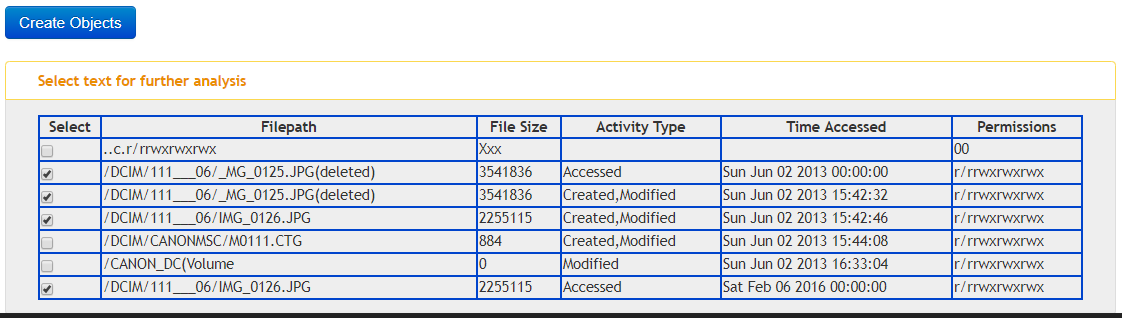
\includegraphics[scale=0.3]{pics/import-table.png}
    
    \begin{itemize}
        \item Possibility to import \textbf{Mactime} files [done]
        \item Pick only relevant files [done]
        \item \texttt{MISPObject} will be created [done]
    \end{itemize}
\end{frame}

\begin{frame}
        \frametitle{Data visualization (MISP 2.4.100/101?)}
    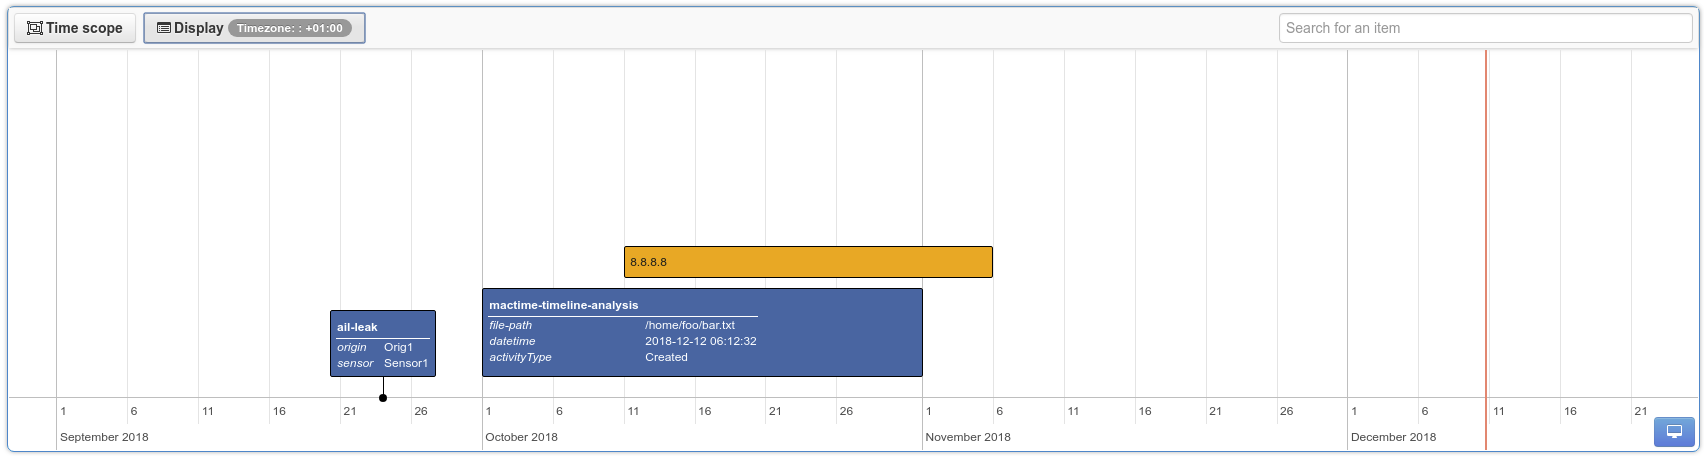
\includegraphics[width=1.0\linewidth]{pics/timeline.png}
    \begin{itemize}
        \item View: start-date only, spanning and search [dev-branch]
        \item Manipulate: Edit, Drag and Expand [dev-branch]
        \item Others: Timezone support [dev-branch]
    \end{itemize}

    \vspace{0.3cm}
    $\rightarrow$ For now [dev-branch], supports up to \textbf{micro-seconds} in the database and up to \textbf{milliseconds} in the web interface.
\end{frame}

\end{document}

